%package list
\documentclass{article}
\usepackage[top=3cm, bottom=3cm, outer=3cm, inner=3cm]{geometry}
\usepackage{graphicx}
\usepackage{url}
%\usepackage{cite}
\usepackage{hyperref}
\usepackage{array}
\usepackage{multicol}
\newcolumntype{x}[1]{>{\centering\arraybackslash\hspace{0pt}}p{#1}}
\usepackage{natbib}
\usepackage{pdfpages}
\usepackage{multirow}
\usepackage{float}
\usepackage[normalem]{ulem}
\useunder{\uline}{\ul}{}


%%%%%%%%%%%%%%%%%%%%%%%%%%%%%%%%%%%%%%%%%%%%%%%%%%%%%%%%%%%%%%%%%%%%%%%%%%%%
%%%%%%%%%%%%%%%%%%%%%%%%%%%%%%%%%%%%%%%%%%%%%%%%%%%%%%%%%%%%%%%%%%%%%%%%%%%%
\newcommand{\csemail}{vmachacaa@unsa.edu.pe}
\newcommand{\csdocente}{Vicente Machaca Arceda}
\newcommand{\cscurso}{Algoritmos y Estructura de Datos}
\newcommand{\csuniversidad}{Universidad Nacional de San Agustín}
\newcommand{\csescuela}{Maestría en Ciencia de la Computación}
\newcommand{\cspracnr}{01}
\newcommand{\cstema}{--}
%%%%%%%%%%%%%%%%%%%%%%%%%%%%%%%%%%%%%%%%%%%%%%%%%%%%%%%%%%%%%%%%%%%%%%%%%%%%
%%%%%%%%%%%%%%%%%%%%%%%%%%%%%%%%%%%%%%%%%%%%%%%%%%%%%%%%%%%%%%%%%%%%%%%%%%%%


\usepackage[english,spanish]{babel}
\usepackage[utf8]{inputenc}
\AtBeginDocument{\selectlanguage{spanish}}
\renewcommand{\figurename}{Figura}
\renewcommand{\refname}{Referencias}
\renewcommand{\tablename}{Tabla} %esto no funciona cuando se usa babel
\AtBeginDocument{%
	\renewcommand\tablename{Tabla}
}

\usepackage{fancyhdr}
\pagestyle{fancy}
\fancyhf{}
\setlength{\headheight}{30pt}
\renewcommand{\headrulewidth}{1pt}
\renewcommand{\footrulewidth}{1pt}
\fancyhead[L]{\raisebox{-0.2\height}{
\includegraphics[width=3cm]{img/logo_unsa}}}
\fancyhead[C]{}
\fancyhead[R]{\fontsize{7}{7}\selectfont	\csuniversidad \\ \csescuela \\ \textbf{\cscurso} }
\fancyfoot[L]{MSc. Vicente Machaca}
\fancyfoot[C]{\cscurso}
\fancyfoot[R]{Página \thepage}


\begin{document}
	
	\vspace*{10px}
	
	\begin{center}	
		\fontsize{17}{17} \textbf{ Práctica \cspracnr}
	\end{center}
	%\centerline{\textbf{\underline{\Large Título: Informe de revisión del estado del arte}}}
	%\vspace*{0.5cm}
	

	\begin{table}[h]
		\begin{tabular}{|x{4.7cm}|x{4.8cm}|x{4.8cm}|}
			\hline
			\textbf{DOCENTE} & \textbf{CARRERA}  & \textbf{CURSO}   \\
			\hline
			\csdocente & \csescuela & \cscurso    \\
			\hline
		\end{tabular}
	\end{table}	
	
	
	\begin{table}[h]
		\begin{tabular}{|x{4.7cm}|x{4.8cm}|x{4.8cm}|}
			\hline
			\textbf{PRÁCTICA} & \textbf{TEMA}  & \textbf{DURACIÓN}   \\
			\hline
			\cspracnr & \cstema & 3 horas   \\
			\hline
		\end{tabular}
	\end{table}
	
	
	\section{Datos de los estudiantes}
	\begin{itemize}
		\item Grupo: 2
		\item Integrantes:
		\begin{itemize}
			\item EDER ALONSO AMPUERO ATAMARI
			\item HOWARD FERNANDO ARANZAMENDI MORALES
            \item JOSE EDISON PEREZ MAMANI
            \item HENRRY IVAN ARIAS MAMANI
		\end{itemize}		
	\end{itemize}
	\section{Algoritmo de Ordenamiento}\label{sec:ejercicios}
    \subsection{caracteristicas}
     \subsection{MergeSort}
    \paragraph{}
    El Merge Sort es un algoritmo recursivo bastante eficiente para ordenar un array, que tiene un orden de complejidad O(nlogn) al igual que Quick Sort. fue desarrollado en 1945 por John Von Neumann.

    El Merge Sort está basado en la técnica de diseño de algoritmos Divide y Vencerás, esta técnica consiste en dividir el problema a resolver en sub problemas del mismo tipo que a su vez se dividirán, mientras no sean suficientemente  pequeños o triviales.
    \begin{figure}[h!]
        \centering
        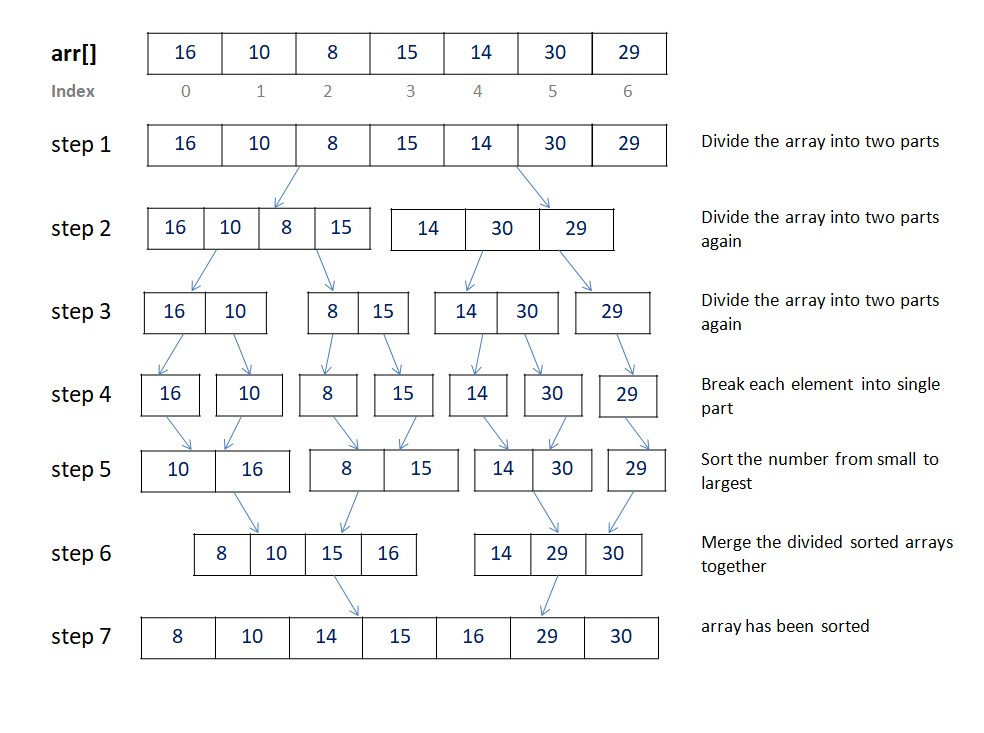
\includegraphics[width=12cm]{img/mergesort.png}
        \caption{Estrategia que sigue algoritmo para ordenar una secuencia S de n elementos}
        \label{fig:mergesort}
    \end {figure}
    \begin{itemize}
        \item Si S tiene uno o ningún elemento, está ordenada.
        \item Si S tiene al menos dos elementos se divide en dos secuencias S1 y S2.
        \item S1 contiene los primeros n/2 elementos y S2 los restantes.
        \item Ordenar S1 y S2, aplicando recursivamente este procedimiento
        \item Mezclar S1 y S2 en S, de forma que ya S1 y S2 estén ordenados
        \item Veamos ahora como sería la estrategia para mezclar las secuencias:
    \end{itemize}
    \paragraph {}
    Se tienen referencias al principio de cada una de las secuencias a mezclar (S1 y S2). Mientras en alguna secuencia queden elementos, se inserta en la secuencia resultante (S) el menor de los elementos referenciados y se avanza esa referencia una posición.
      \subsubsection{Gráfica MergeSort}
        \begin{figure}[h!]
            \centering
            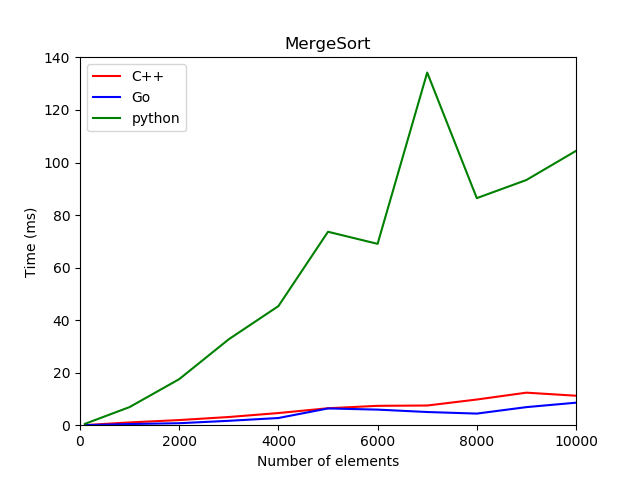
\includegraphics[width=12cm]{img/mergeSort_1.png}
            \caption{Estrategia que sigue algoritmo para ordenar una secuencia S de n elementos}
            \label{fig:mergesort}
        \end {figure}
        \begin{figure}[h!]
            \centering
            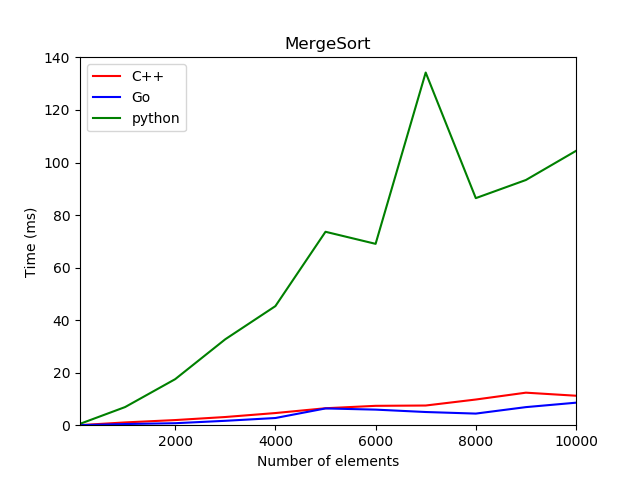
\includegraphics[width=12cm]{img/mergeSort_2.png}
            \caption{Estrategia que sigue algoritmo para ordenar una secuencia S de n elementos}
            \label{fig:mergesort}
        \end {figure}

    \subsection{QuickSort}

    \subsection{HeapSort}
            \begin{figure}[h!]
            \centering
            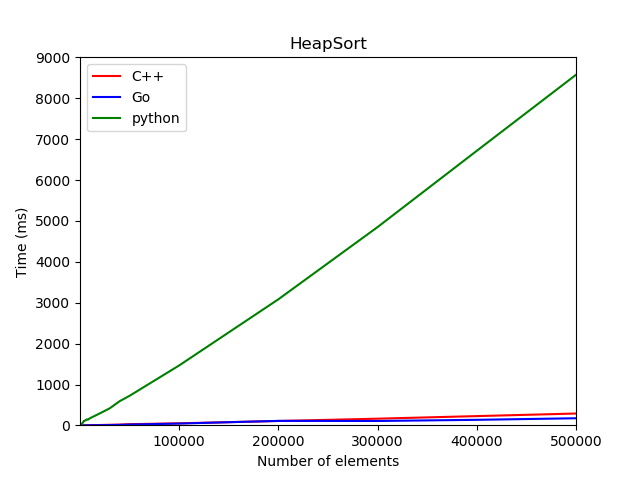
\includegraphics[width=12cm]{img/HeapSort_1.png}
            \caption{Estrategia que sigue algoritmo para ordenar una secuencia S de n elementos}
            \label{fig:mergesort}
        \end {figure}
                \begin{figure}[h!]
            \centering
            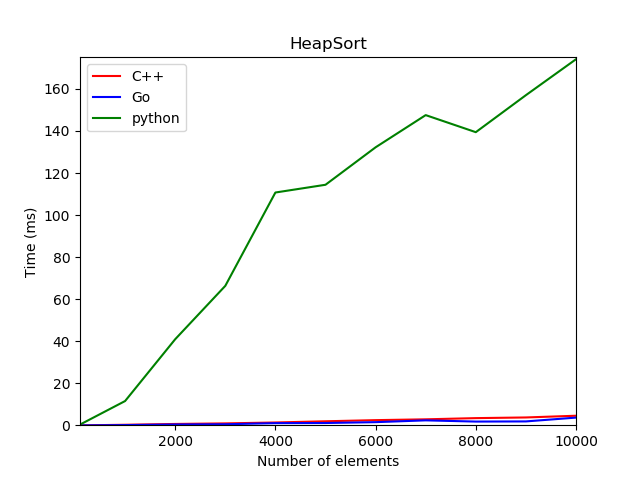
\includegraphics[width=12cm]{img/HeapSort_2.png}
            \caption{Estrategia que sigue algoritmo para ordenar una secuencia S de n elementos}
            \label{fig:mergesort}
        \end {figure}
    \subsection{TreeSort}
    La clasificación de árbol es un algoritmo de clasificación que se basa en la estructura de datos del árbol de búsqueda binaria. Primero crea un árbol de búsqueda binario a partir de los elementos de la lista o matriz de entrada y luego realiza un recorrido en orden en el árbol de búsqueda binario creado para ordenar los elementos.
        \subsubsection{CostoComputacionla}
        \subsubsection{Resultado de las pruebas}
        \begin{figure}[h!]
            \centering
            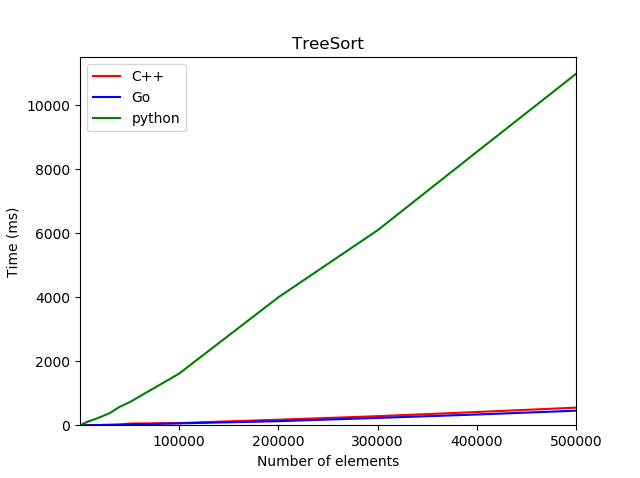
\includegraphics[width=12cm]{img/treeSort_1.png}
            \caption{Estrategia que sigue algoritmo para ordenar una secuencia S de n elementos}
            \label{fig:mergesort}
        \end {figure}        
        \begin{figure}[h!]
            \centering
            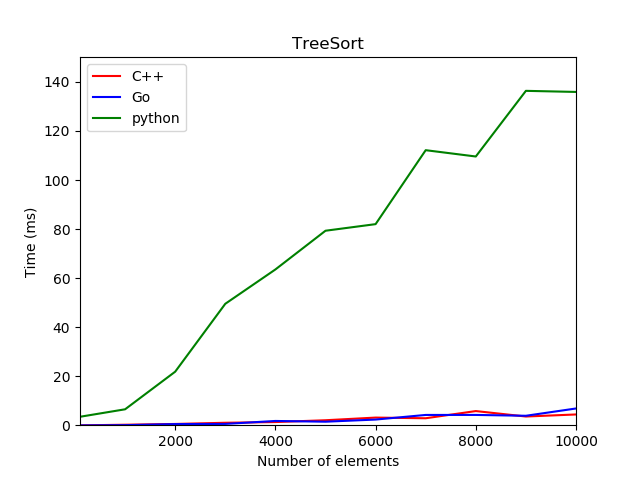
\includegraphics[width=12cm]{img/treeSort_2.png}
            \caption{Estrategia que sigue algoritmo para ordenar una secuencia S de n elementos}
            \label{fig:mergesort}
        \end {figure}

	
	%\clearpage
	%\bibliographystyle{apalike}
	%\bibliographystyle{IEEEtranN}
	%\bibliography{bibliography}
		
	
\end{document} 